\chapter{Introduction}
\label{chapter:introduction}

As neuromorphic computing becomes ever more popular, many applications for such systems emerge and make use of its hardware's advantages over traditional computers.
But to do so one must be familiar with a system as it often differs in many ways from common system architectures.
As a result programing for such systems can feel odd to new users as they need to abandon some familiar techniques and acquire new skills.
This understandably is a hurdle for many users and also initially takes a significant amount of time. 
The more a system's programming abandons common elements of programming which users are accustomed to the more this can become a problem.
Not only do fewer users take the initiative of writing for such systems but also can code easily get confusing, hard to debug and even ineffective.

An example of this is the current state of programming for the plasticity processing unit of the Hicann-DLS.
It is responsible for applying learning rules to neural systems on the Hicann-DLS and resembles a common processor which was extended for this cause.
Despite basic programming still being the same for this processor it differs for creating the mentioned learning rules.
Although these are still programmed in C a user needs to use a set of functions and predefined variables while at the heart of this is basic assembly programming.
This was done to include users unskilled in assembly who want to write programs for the PPU.
This lead to PPU programs having a distinct look and feel that is only in some regards similar to C but feels like being pushed back to the origins of computing; for example reading out the value of a variable need unhandy workarounds and accessing memory is a repetitive set of program lines.
The main reason we feel so reluctant when it comes to outdated programming are compilers.

Since the early stages of computing, compilers have developed towards a standard tool in everyday programming but at the same time became more of a black box that transforms a program into an executable file.
For this reason it may be difficult for some users to abandon such convenience and go back to low-level programming.

But luckily the PPU is not completely without compiler support as basic computing is support but new features of the PPU are only usable on a low level.
This could still cause major inconvenience for users as these features are necessary to implement learning rules for synapses which are themselves elementary to neuromorphic programming.
As of now users are forced under these circumstances to mix high-level programming with very low-level programming.
Of course this possibly leads to a series of problems as users have to adapt to this atypical style of programming.
At worst this can even lead to ineffective programs --- although performance is important for neuromorphic programming and the main advantage of the PPU --- and demand an unreasonable amount of time and work to achieve simple results.

\begin{wrapfigure}{R}{0.4\textwidth}
    \centering
    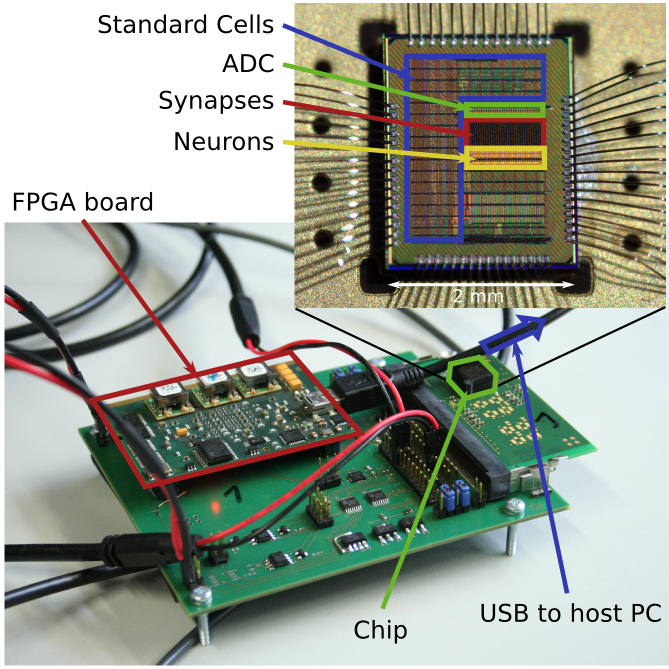
\includegraphics[width=0.4\textwidth]{pictures/Fig1.png}
    \caption{\label{fig:dlsboard} set-up of a HICANN-DLS test system}
\end{wrapfigure}
Although this makes it obvious that compiler support is desirable the reason for the PPU not having compiler support is the custom nature of the processor architecture, which was developed solely for the BrainScaleS system and the HICANN-DLS.
It could be classified as an application specific instruction set architecture (ASIP) which is an intermediate form between general purpose processors and application specific integrated circuits (ASIC).
Such architectures offer a partly customized instruction set architecture (ISA) that is optimized for certain applications.

Hence the only way to support complete high-level programming is adding compiler support for the PPU's ISA.

Not only would this permit full C-style high-level programming when working on the PPU but could also include code optimization and code debugging.
We therefore aim to achieve ``full'' compiler support of the PPU's hardware and make programming easier which ultimately should open the platform for new users, simplify programming for existing users and possibly accelerate performance on the PPU.
At some point compiler support could also lead to automatic code generation which then could allow for implementation of high-level languages.
Ultimately the goal should be that users do not need to code for the PPU itself but create plasticity rules in existing program environments that translate this ``meta-code'' into PPU programs.
Obviously this calls for optimization of PPU code and although this could be done by developers specifically for the PPU it is far easier and likely more efficient to utilize existing optimization techniques that are built into virtually every compiler.

This thesis will focus on the way to achieve mentioned compiler support and briefly explain the process itself.
As fundamental knowledge of both processors and compilers is needed along the way it will start with a very basic introduction to both topics and go into detail for the processor and compiler that were used later on.
This may not render additional literature obsolete but should explain the basic concepts to an extend which is sufficient.
Afterwards the process of extending the compiler is explained and the result as well as test cases of this presented.
The thesis will conclude in a resume and give an outlook to the future applications and development of the compiler.

